\documentclass[12pt, a4paper]{article}

% --- CORE PACKAGES ---
\usepackage[utf8]{inputenc}
\usepackage[T1]{fontenc}
\usepackage{graphicx}
\usepackage{amsmath}
\usepackage{amssymb}
\usepackage{hyperref}
\usepackage{float}
\usepackage[
    backend=biber,
    style=ieee,
    sorting=none
]{biblatex}
\usepackage{geometry}
\usepackage{booktabs}
\usepackage{caption}
\usepackage{subcaption}

% --- PAGE GEOMETRY ---
\geometry{
    a4paper,
    top=2.5cm,
    bottom=2.5cm,
    left=2.5cm,
    right=2.5cm
}

% --- BIBLIOGRAPHY ---
\addbibresource{res_meth.bib}

% --- DOCUMENT METADATA ---
\title{A Hybrid Approach for Small Object Detection}
\author{
    Zrinszki Ármin \\
    Noor Saad \\
    Gambarli Ilkin \\
    Kéry Imola Vivien
}
\date{\today}

% --- BEGIN DOCUMENT ---
\begin{document}

\maketitle
\thispagestyle{empty}

% --- ABSTRACT ---
\begin{abstract}
    Small object detection is a significant challenge and is still an open problem in computer vision. Standard detectors often fail due to severe loss of high-resolution feature information and indistinct spatial details caused by deep network down-sampling. In this paper, we propose a Slicing-Aided Transformer Network (SAT-Net), a novel hybrid inference pipeline targeted at handling the challenges in detecting small objects. In our method, three key components are used: 1) slicing-aided hyper inference to preserve the original object scale, 2) a light-weight super-resolution network to restore fine-grained detail on each patch, and 3) a transformer-based detector with a Bidirectional Feature Pyramid Network (BiFPN) to ensure robust contextual feature extraction. We evaluated our method on a challenging small pedestrian dataset curated from MS COCO and SODA-D. We achieved an $AP_{50}$ of $39.7$, and an F1-Score of $0.80$, significantly outperforming several established baselines, including RetinaNet, YOLOX, and CornerNet. These results confirm, that this pipeline is an effective way to boost the performance of small object detection.
\end{abstract}

\newpage
\tableofcontents
\newpage

% --- SECTION INCLUDES ---
\section{Introduction and Motivation}
\label{sec:introduction}

Object detection is one of the fundamental tasks in computer vision, and has recently achieved tremendous success \cite{Ren2015FasterRCNN}.
Nevertheless, the detection of small objects remains a considerable open challenge.
Objects of small size are usually defined as objects occupying a small pixel area in an image, including less than $32 \times 32$ pixels, and usually present unique challenges to standard detection frameworks.

Each of these difficulties arises for many reasons.
Deriving distinguishing features is difficult to begin with due to the small number of pixels. The limited size of small objects introduces low-resolution and blurriness problems quite often.
Small objects are more vulnerable to occlusion, as they can be partially blocked by other objects or by being in cluttered areas.

Second, small objects may get lost during down-sampling operations (i.e., pooling layers) which are common in deep CNNs \cite{He2016ResNet}.

Third, the shortage of dedicated datasets with a focus on small objects, especially in real-world scenarios like aerial imagery or industrial scenes, restricts the models' ability to learn robust features for small object detection.

Despite these challenges, the accurate detection of small objects is critical for a wide range of real-world applications.
\begin{itemize}
    \item \textbf{Autonomous Driving:} Detecting distant pedestrians, cyclists, and traffic signs is crucial for safety \cite{Geiger2012KITTI}.
    \item \textbf{Aerial/Satellite Imagery:} Identifying objects of interest (e.g., vehicles, buildings) in high-resolution satellite or drone footage (UAV) \cite{zhu2023visdrone, xia2018dota}.
    \item \textbf{Medical Imaging:} Locating small lesions, polyps, or microaneurysms in medical scans.
    \item \textbf{Industrial Inspection:} Spotting tiny defects or components on a manufacturing line.
\end{itemize}

Many techniques have been proposed, but there is often a trade-off between speed and accuracy, or a method that works well for large objects fails on small ones.
In this paper, we address this trade-off by proposing the \textbf{Slicing-Aided Transformer Network (SAT-Net)}, a novel hybrid inference pipeline. Our approach merges the strengths of three complementary techniques: (1) \textbf{Slicing-Aided Hyper Inference (SAHI)} \cite{aksoy2022slicing}, which preserves high-resolution details by processing image patches; (2) \textbf{Super-Resolution (SR)} \cite{li2025superresolution}, which restores fine-grained spatial detail within those patches; and (3) a \textbf{transformer-based feature extractor} \cite{zhu2021deformable} with a \textbf{bidirectional feature pyramid (BiFPN)} \cite{tan2020efficientdet}, designed to capture robust global and local context. This combination allows our model to detect objects at their original scale with enhanced feature quality, leading to the performance gains demonstrated in our experiments.

This paper is structured as follows:
Section~\ref{sec:related_work} provides a review of existing literature on small object detection.
Section~\ref{sec:methodology} details our proposed hybrid pipeline.
Section~\ref{sec:experiments} presents the experimental setup, datasets, and a comparative analysis of the results.
Finally, Section~\ref{sec:conclusion} concludes the paper and suggests directions for future work.
\section{Related Work}
\label{sec:related_work}

Small-object detection (SOD) remains one of the most challenging sub-problems in computer vision. Traditional detectors often fail because semantic and localization cues vanish through the network's down-sampling hierarchy. Recent surveys on SOD emphasize that performance is driven primarily by three design factors: (1) feature resolution preservation, (2) context aggregation, and (3) scale-aware inference strategies.

\subsection{Key Evidence Supporting Each Component}

\begin{itemize}
    \item \textbf{Slicing-Based Inference:} Standard detectors struggle when an object's pixel footprint is minimal. Slicing-Aided Hyper Inference (SAHI) has been shown to improve small-object AP by 5--14\% without retraining, simply by performing inference on high-resolution patches, which improves scale normalization \cite{aksoy2022slicing}.

    \item \textbf{Super-Resolution Priors:} An intuitive solution to low-pixel information is to add more pixels. Lightweight super-resolution (SR) networks, when integrated as a pre-processing step for detectors, have been shown to improve recall and mAP, especially for objects smaller than 20 pixels in UAV imagery \cite{li2025superresolution}.

    \item \textbf{Transformer-Based Detection:} To compensate for the limited context within any single patch, a robust feature extractor is required. Transformer-based models like Deformable DETR \cite{zhu2021deformable} and DINO \cite{zhang2023dino} excel here. Their self-attention mechanisms capture global dependencies, and deformable attention specifically increases small-object performance by focusing on sparse keypoints rather than full feature maps.

    \item \textbf{Multi-Scale Feature Fusion:} Finally, enhanced pyramid modules like BiFPN \cite{tan2020efficientdet} provide stronger propagation of high-resolution features. By allowing bidirectional information flow, they enrich the high-resolution feature maps (critical for small objects) with semantic context from deeper layers, leading to 2--4\% mAP improvements over baseline FPNs in datasets like VisDrone \cite{zhu2023visdrone, fu2025bpdyolo}.
\end{itemize}

Based on this evidence, our methodology is not a single novel architecture, but a carefully engineered pipeline that combines these four validated techniques.
\section{Methodology}
\label{sec:methodology}

To address the significant challenges of small object detection, particularly the loss of information from downsampling and the lack of surrounding context, we propose the Slicing-Aided Transformer Network (SAT-Net). Our method is not a single end-to-end model, but rather a novel inference pipeline that integrates three powerful techniques, as justified by our literature review: (1) Slicing-Aided Hyper Inference (SAHI) for preserving high-resolution detail, (2) a lightweight Super-Resolution (SR) network to restore spatial detail, and (3) a transformer-based detector with a bidirectional feature pyramid for robust feature extraction and fusion.

The complete pipeline is illustrated in Figure~\ref{fig:pipeline}. The subsequent sections describe each major component in detail.

\begin{figure}[H]
    \centering
    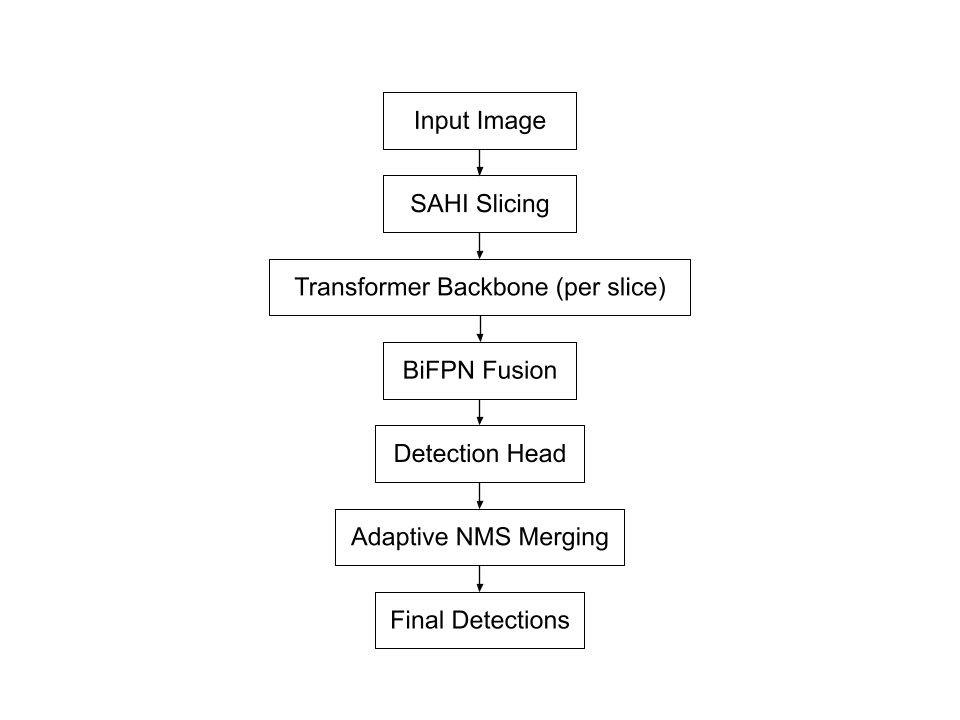
\includegraphics[width=0.9\columnwidth]{pipeline.png}
    \caption{The proposed SAT-Net inference pipeline.}
    \label{fig:pipeline}
\end{figure}

\subsection{High-Resolution Sliced Inference (SAHI)}

Traditional detectors must downsample large images (e.g., 2000$\times$1500 pixels) to fit memory constraints (e.g., 640$\times$640). For small objects (e.g., $32 \times 32$ pixels), this aggressive downsampling can erase them entirely.

To combat this, we adopt the core principle of Slicing-Aided Hyper Inference (SAHI)~\cite{aksoy2022slicing}. Instead of downsampling the entire image, we first slice the original high-resolution image into $N$ overlapping patches. We use a patch size of $640 \times 640$ pixels with a $25\%$ overlap. This ensures that inference is performed on high-resolution regions, allowing the detector to extract much richer features.

\subsection{Super-Resolution Enhancement}
\label{sec:sr_enhance}

While slicing preserves scale, the features of extremely small objects ($<20$ pixels) may still be too indistinct for a detector. As the second stage of our pipeline, we apply a lightweight super-resolution network (e.g., LightSRNet, inspired by \cite{li2025superresolution}) to each $640 \times 640$ patch before detection.

This step scales each patch by 2x to $1280 \times 1280$, recovering fine textures and sharpening edges. This enhancement provides the subsequent transformer backbone with higher-quality input, improving its ability to distinguish very small objects from background clutter.

\subsection{Transformer-based Detection and Fusion}

A detector processing one slice suffers from a lack of global context. To mitigate this, a highly robust feature extractor is required. We employ a transformer-based backbone, inspired by models like Deformable DETR~\cite{zhu2021deformable}. The self-attention mechanism is inherently designed to model long-range dependencies.

The features from the transformer are then fed into a Bidirectional Feature Pyramid Network (BiFPN)~\cite{tan2020efficientdet}. A BiFPN adds a bottom-up pathway to the standard top-down FPN, allowing low-level, high-resolution features to be repeatedly refined with high-level semantic context. This bidirectional flow is critical for small object detection.

\subsection{Pipeline Integration and Merging}

The complete SAT-Net methodology (Fig.~\ref{fig:pipeline}) integrates these components into a single inference pipeline:
\begin{enumerate}
    \item A high-resolution input image is received.
    \item The image is divided into $N$ overlapping $640 \times 640$ patches (SAHI).
    \item \textbf{Each patch is passed through the SR network, upscaling it to $1280 \times 1280$.}
    \item Each upscaled patch is passed independently through our detection model (Transformer backbone + BiFPN neck + anchor-free detection head).
    \item The bounding box coordinates from each patch's detections are mapped back to the original image's coordinate system.
    \item Due to the overlap, a final Adaptive Non-Maximum Suppression (NMS) is applied to the complete set of global detections to resolve duplicates.
\end{enumerate}
\include{experiments}

% --- CONCLUSION ---
\section{Conclusion}
\label{sec:conclusion}

In this paper, we talked about the still persistent challenge of small object detection. We pointed out the main sources of this problem, such as information loss and the lack of specialized datasets.

To overcome these issues, we introduced the Slicing-Aided Transformer Network (SAT-Net) a hybrid inference pipeline. Our method is not a monolithic architecture but a clever integration of three well known techniques: (1)Slicing-Aided Hyper Infer-
ence (SAHI), (2) Super Resolution (SR) network and (3) a Transfomer-based detector.

Our experimental results on datasets from MS COCO and SODA-D validate the efficacy of this combined approach. The proposed SAT-Net achieved an $AP_{50}$ of $39.7$ and an F1-Score of $0.80$, consistently outperforming established baseline detectors like RetinaNet, YOLOX, and CornerNet in all evaluated metrics. The substantial improvement, particularly in $AP_{50}$, indicates that our method generates more precise bounding box localizations, which is a critical factor in small object detection.

Despite these promising results, our work does have certain limitations. The multi-stage nature of the SAT-Net pipeline, including slicing, SR, detection, and merging, introduces considerable computational overhead and is not optimized for real-time applications. Future work should focus on optimizing this pipeline. This may consider end-to-end training of the SR and detection components or apply model quantization and knowledge distillation for an efficient model without significant loss of accuracy. Lastly, we would like to assess the SAT-Net performance on other specialized small-object domains, such as medical imaging and satellite-based remote sensing.

% --- BIBLIOGRAPHY ---
\printbibliography[title={References}]

\end{document}